%%%%%%%%%%%%%%%%%%%%%%%%%%%%%%%%%%%%%%%%%%%%%%%%%%%%%%%%%%%%%%%%%%%%%%%%%%%%%%%%%%%%%%%%%%%%%%%%%%%
% Chapter 8 -> PHLOWER Experiments and Results
% Author: Mingbo Cheng
%%%%%%%%%%%%%%%%%%%%%%%%%%%%%%%%%%%%%%%%%%%%%%%%%%%%%%%%%%%%%%%%%%%%%%%%%%%%%%%%%%%%%%%%%%%%%%%%%%%
\chapter{PHLOWER Experiments \& Results}
\label{chapter:PHLOWER_bench}
\graphicspath{{chapter8/figs}}

%%TODO
%% Order CAN BE technical experiment and result, followed by biological experiment and result.

In the previous chapter, we introduced our computational method, PHLOWER, for trajectory inference in single-cell multimodal data. In this chapter, we outline the technical experimental framework~(\sref{PHLOWER_bench:tech_exp}) utilized in this thesis to validate our trajectory inference methods and subsequently present the results~(\sref{PHLOWER_bench:tech_out}). Within the experimental framework, we first introduce the synthetic benchmarking dataset. Following that, we discuss the four evaluation metrics used for measuring topology recovery, cell location, branch allocation accuracy, and branch point allocation accuracy, drawing from the comprehensive evaluation framework dynverse. Subsequently, we delve into the execution of competing methods for the benchmarking process, comparing against 11 state-of-the-art methods. In the results section, we present the outcomes of the benchmarking evaluation.

Next, we introduce the biological validation design~\srefp{PHLOWER_bench:bio_exp}. specifically the kidney organoid data preparation and experiment design. Next, we showcase the biological validation using the kidney organoid data. Following this, we present the statistical methods employed in the chapter~\srefp{PHLOWER_bench:statistical}. Finally, we conclude the chapter by discussing the strengths of PHLOWER~\srefp{PHLOWER_bench:discussion}.



\section{Technical Experiments}
\label{PHLOWER_bench:tech_exp}
In this section, we initially present the algorithm for creating simulated data~(\sref{PHLOWER_bench:sim}). Following that, we elaborate on four trajectory inference evaluation metrics~(\sref{PHLOWER_bench:metrics}). Subsequently, we provide detailed descriptions for the execution of each method~(\sref{PHLOWER_bench:exe}).

\subsection{Simulated Data}
\label{PHLOWER_bench:sim}
To test the power of PHLOWER in the detection of multiple branches trees, we generate 10 simulated data sets using diffusion-limited aggregation trees (DLA tree)~\citep{witten1981diffusion} as proposed in PHATE~\citep{moon2017phate}. For this, we use a Gaussian noise parameter of 5 and vary the parameter n\_branch, which controls the number of branches in the trees, from 3 to 12. This generated trees with 5 to 18 branches.  For every data, we generate \num{3000} points and \num{100} features. Of note, we use the same data as evaluated in PHATE as data with 10 branches. Next, we run PHATE to visualize the branches, with which we can future construct ground truth for dynverse benchmarking~\alref{alg:DLA}~\trefp{tab:DLA_trees}.

\begin{figure}[!h]
	\centering
	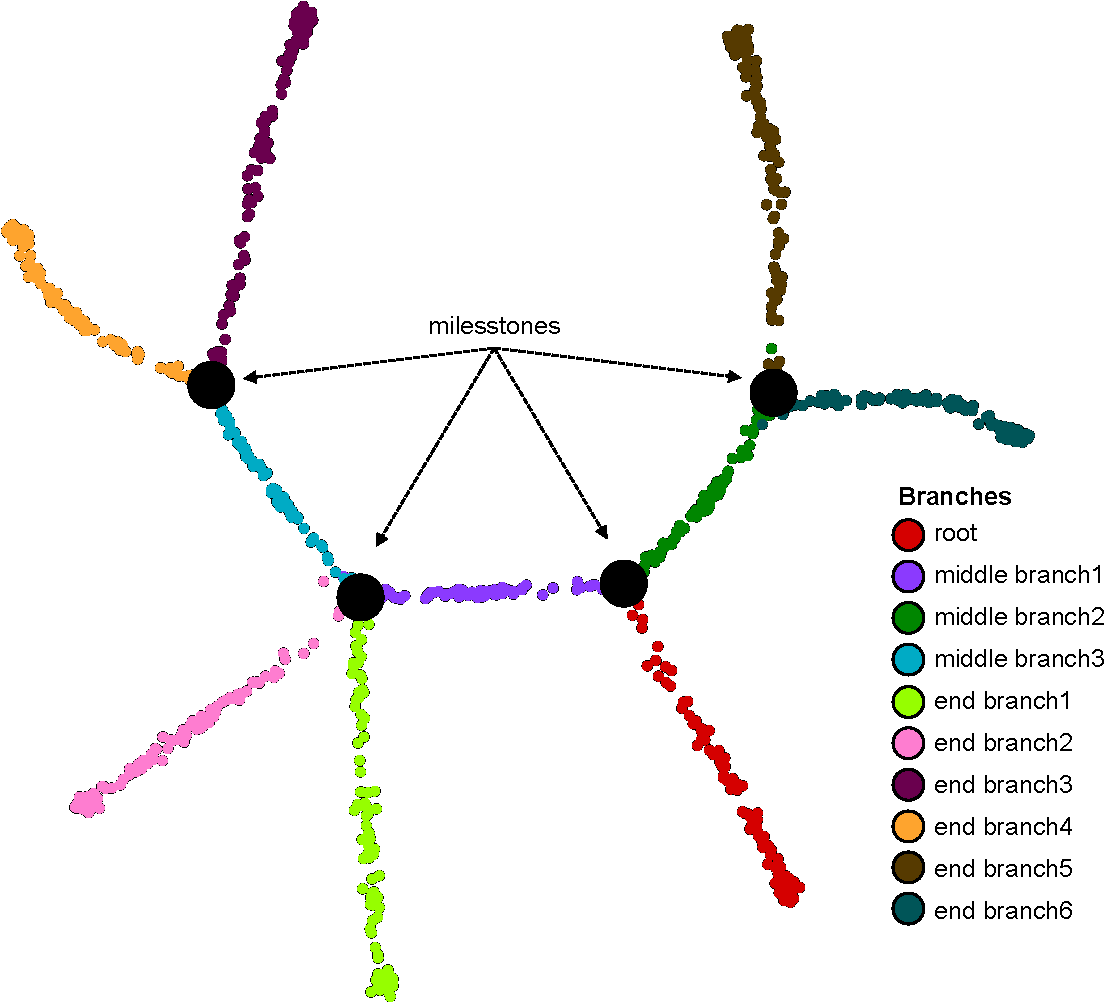
\includegraphics[width=0.45\textwidth]{DLA_example/fig}
	\vspace{0.1cm}
	\caption[DLA tree ground truth example]{DLA tree ground truth example embedded with PHATE.}
	\label{fig:DLA_example}
\end{figure}


Next, we reformat this data to be used within the trajectory benchmarking framework dynverse~\citep{saelens2019comparison} by using dynwrap. In short, dynverse needs detailed information of the branches, branches points and association of cells within a branch.  To do so, we need to find the branching points of the DLA tree. First, we perform PHATE on the DLA high dimensional data to get embedding with 2 dimensions. We only consider embeddings, where the tree structure is preserved. Next, we find the branching points by finding 2 nearest neighbors of two branches. With these branching points, we created the branch backbones needed by dynverse. We calculate am association of each data point to a branching point (milestone percentage) by calculating the euclidean distance between the points related to each branch. See DLA tree with 10 branches example \fref{fig:DLA_example}.

\begin{table}[!ht]
	\footnotesize
	\centering
	\begin{tabular}{cccc|ccp{0.15\linewidth}}
		\toprule
		\multicolumn{4}{c}{Paramters} & \multicolumn{2}{c}{Output}\\
    {\textbf{nbranches}} & {\textbf{npoints}} & \textbf{ndimension} & {\textbf{noise $\sigma$}}  &{\textbf{\#branches}}  & {\textbf{\#branching point}}\\
		\midrule
    \textbf{{3}}   & \num{3000} & \num{100} & 5 & \num{5}  & \num{2} \\
    \textbf{{4}}   & \num{3000} & \num{100} & 5 & \num{7}  & \num{3} \\
    \textbf{{5}}   & \num{3000} & \num{100} & 5 & \num{5}  & \num{2} \\
    \textbf{{6}}   & \num{3000} & \num{100} & 5 & \num{9}  & \num{4} \\
    \textbf{{7}}   & \num{3000} & \num{100} & 5 & \num{11} & \num{5} \\
    \textbf{{8}}   & \num{3000} & \num{100} & 5 & \num{13} & \num{5} \\
		\textbf{{9}}   & \num{3000} & \num{100} & 5 & \num{14} & \num{6} \\
    \textbf{{10}}  & \num{1440} & \num{60}  & 5 & \num{10} & \num{4} \\
		\textbf{{11}}  & \num{3000} & \num{100} & 5 & \num{18} & \num{9} \\
		\textbf{{12}}  & \num{3000} & \num{100} & 5 & \num{16} & \num{8} \\
		\bottomrule
	\end{tabular}
	\vspace{0.1cm}
	\caption[TI DLA trees synthetic data.]{TI DLA trees synthetic data.}
	\label{tab:DLA_trees}
\end{table}


\begin{algorithm}
\caption{Diffusion-Limited Aggregation Tree Generation}
\label{alg:DLA}
\Input{
	$n$, number of samples\\
 	$d$, number of dimensions\\
 	$b$, number of branches\\
 	$\sigma$, gussian noise standard deviation parameter\\
 }
    \textbf{seed random number generator}\\
    $s \gets \lfloor\frac{n}{b}\rfloor$\Comment*[r]{Number of steps}
    $u \sim \textbf{Uniform}(0,1)\in\mathbb{R}^{s \times d}$\\
    $M \gets \textbf{Cumsum}(-1 + 2 \times u)$\\
    \While{$I \gets 1$ to $b$}
    {
         $i \gets \textbf{Random}\{1,2,\cdots, s\}$\\
         $u_2 \sim \textbf{Uniform}(0,1)\in\mathbb{R}^{s \times d}$\\
         $M_2 \gets \textbf{Cumsum}(-1 + 2 \times u_2)$\\
        $M \gets \begin{bmatrix}M \\\\
            M_2 +\left[\begin{array}{c}
                M(i, :)\\
                M(i, :)\\
                \vdots\\
                M(i, :)\\
        \end{array}\right]_{s\times d} \end{bmatrix}$\\
    }
    $C \gets (\underbrace{1,1,\cdots, 1}_{s \text{ times}}, \underbrace{2,2,\cdots, 2}_{s \text{ times}},  \cdots\cdots, \underbrace{b,b,\cdots, b}_{s \text{ times}})$\\
    $\epsilon \sim \mathcal{N}(0, \sigma^2)\in\mathbb{R}^{n\times d}$\\
    $M \gets M + \epsilon$\\
    \Return \{$M$, $C$\}\\
\end{algorithm}

%3000, \num{100}, br, 5.
%3-12

\subsection{Evaluation of Trajectory Inference}
\label{PHLOWER_bench:metrics}
% dynverse benchmarking selected metrics description
The simulated data for trajectory inference. We first described the data source and pre-processing for single cell multi-modal data, next we show how to simulate data for trajectory inference.
\begin{figure}[!h]
	\centering
	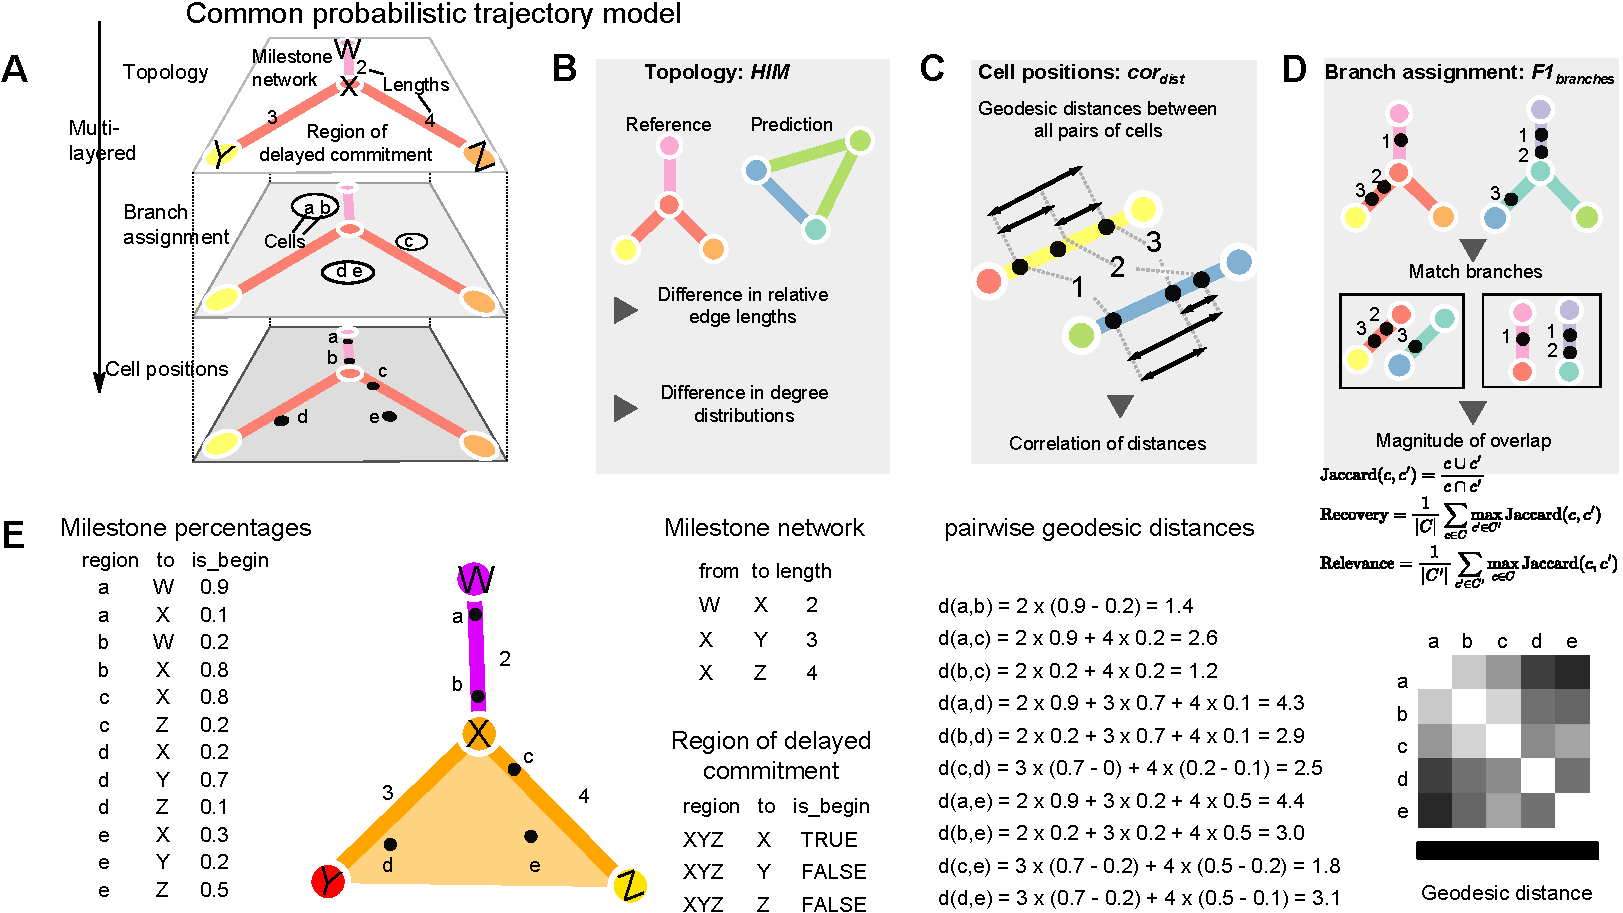
\includegraphics[width=0.95\textwidth]{dynverse_metrics/fig}
	\vspace{0.1cm}
	\caption[Dynverse metrics]{ \textbf{A)} dynverse metrics. Dynverse has established three significant metrics here, each evaluating the excellence of various facets of the trajectory. \textbf{B)} The HIM score gauges the resemblance between the two topologies, considering variations in edge lengths and degree distributions. \textbf{C)} $cor_{dist}$ measures the similarity in cellular positions between two trajectories by computing the correlation among pairwise geodesic distances. \textbf{D)} The $F1_{branches}$ evaluates the likeness in the allocation of cells to branches. \textbf{E)} The geodesic distances were computed on a small example trajectory. This toy example consists of four milestones (W to Z) and five cells (a to e). The milestone network, milestone percentages, and regions of delayed commitment corresponding to the toy trajectory were transformed into the common trajectory model. The calculations were performed to determine pairwise geodesic distances, and a heatmap representation was generated to visually depict these distances.}
	\label{fig:dynverse_metrics}
\end{figure}

To facilitate direct comparability between outputs from various methods, dynverse\citep{saelens2019comparison} designed a unified probabilistic model to represent trajectories from all potential sources\fref{fig:dynverse_metrics}A. In this model, the comprehensive topology is depicted by a network of `milestones', and cells are positioned within the space defined by each connected set of milestones. In dynverse evaluation, a trajectory is conceptualized as a model with multiple layers of abstraction. The highest-level abstraction is the topology, which encompasses information about the paths each cell can traverse from its starting point. Deeper abstractions involve the mapping of each cell to a specific branch within this network, as well as the position (or ordering) of each cell within these branches. Internally, the topology is represented by the milestone network and regions of delayed commitment, while branch assignment and cellular positions are captured by milestone percentages \fref{fig:dynverse_metrics}A.

\begin{description}
	\item[Benchmarking Structure Similarity]
	The Hamming–Ipsen–Mikhailov(HIM) metric~(\fref{fig:dynverse_metrics}B) utilizes the two weighted adjacency matrices of the milestone networks as input, with weights assigned based on edge length. It combines the normalized Hamming distance, providing insights into differences in edge lengths, and the normalized Ipsen–Mikhailov distance, evaluating the similarity in degree distributions. The Ipsen–Mikhailov distance includes a parameter $\gamma$, set at 0.1 to ensure comparability of scores across datasets. The HIM metric is a linear combination of these components.

	\item[Benchmarking Location of Cells]
	The $cor_{dist}$ metric~(\fref{fig:dynverse_metrics}C) measure the correlation between geodesic distances, which is based on the observation that when a cell's position is identical in both the reference and the prediction, its relative distances to all other cells in the trajectory should also be identical. To calculate $cor_{dist}$, dynverse initially simples \num{100} waypoint cells in both the prediction and the reference dataset, employing stratified sampling across various milestones, edges, and regions of delayed commitment. This sampling is weighted by the number of cells in each collection. Subsequently, it computes the geodesic distances between the union of waypoint cells from both datasets and all other cells. The calculation of geodesic distance takes into account the location of the two cells within the trajectory and is weighted by the length of the edge in the milestone network. Finally, $cor_{dist}$ is defined as the Spearman rank correlation between the distances of both datasets.

	\item[Bechmarking Branches Allocation]
	For branch assignment comparison~(\fref{fig:dynverse_metrics}D), measure the The F1 between branch assignments. Dynverse employs an F1 score, a metric commonly utilized for comparing biclustering methods. To compute this score, it initially determines the similarity of all pairs of branches between the two trajectories using Jaccard similarity. Subsequently, it defines 'Recovery' (respectively 'Relevance') as the average maximal similarity of all branches in the reference dataset (respectively prediction). The $F1_{branches}$ is then established as the harmonic mean between Recovery and Relevance.

	\begin{equation}
	\label{eqn:corrdist}
	\begin{aligned}
	& \text{Jaccard}(c, c')  = \frac{c\cup c'}{c\cap c'} \\
	& \text{Recovery} = \frac{1}{|C|}\sum_{c\in C} \max_{c'\in C'} \text{Jaccard}(c, c') \\
	& \text{Relevance} = \frac{1}{|C'|}\sum_{c' \in C'} \max_{c\in C} \text{Jaccard}(c, c')\\
	& F1 = \frac{2}{\frac{1}{\text{Recovery}} + \frac{1}{\text{Relevance}}}
	\end{aligned}
	\end{equation}
	where $C$ and $C'$ represent two cell clusters, in this context, signifying clusters that include cells belonging to a specific branch.
	\item[Benchmarking Branch Points Allocation]
	Similar to $F1_{branches}$, other than mapping cells to edges, the $F1_{milestones}$, namely the F1 between milestone assignments, cells are mapped towards the nearest milestone, i.e. the milestone with the highest milestone percentage.
\end{description}


\subsection{Execution of Trajectory Inference}
\label{PHLOWER_bench:exe}
% List how to install and run the competing methods
% how to set up dynverse environment
We first, install dyno(0.1.2) which includes some competing methods of wrapping. To do this, we use devtools::install\_github(``dynverse/dyno'') which includes the dynverse packages dynwrap(1.2.3),  dynmethods(1.0.5.9000), dynplot(1.1.2) and dynfeature(1.0.0). For PHLOWER and STREAM wrapping, we followed tutorial~\url{https://dynverse.org/developers/creating-ti-method/}. For this, we clone dynclipy(0.1) code from~\url{https://github.com/dynverse/dynclipy} and use ``pip install .'' to install the package.

\begin{description}
	\item[PHLOWER] As PHLOWER utilizes STREAM for visualization, the wrapping to dynverse follows a similar approach to STREAM. To construct the stream tree structure, PHLOWER initially allocates each cell to the tree branches. This is achieved by considering the location of all edges associated with a vertex and using the mean value in the cumulative trajectory embedding space. Given that each edge can have multiple coordinates in the cumulative trajectory space, the median value is employed as the edge coordinate for inferring the cell coordinate. Subsequently, PHLOWER identifies the nearest branch to which a cell is close and assigns the cell to the respective branch. For cells that remain unvisited during the random walk, their k(default 5) nearest neighbors in the original space are used to approximately represent the cumsum coordinate. With this information, we can seamlessly integrate our tree into STREAM.

	\item[Celltree]
	celltree has been wrapped in dynmethods in~\url{https://github.com/dynverse/ti\_celltree\_vem}. However, the cellTree source code normalization function ``.normalise.data'' would not work with negative values. We check out cellTree(1.27.0) source code from~\url{https://git.bioconductor.org/packages/cellTree} and adjust the ``.normalise.data'' function to use 0-1 normalization as the data output for the downstream inference process and recompile cellTree package as the input of dynmethods wrapper. We re-wrap ti\_celltree\_vem code to use the call new cellTree package to be a new wrapper method\_celltree\_vem. And pass method\_celltree\_vem function to dynwrap function infer\_trajectory to infer the trajectory.

	\item[ElPiGraph]
	ElPigraph has been wrapped in dynmethods, we just pass the ti\_elpigraph function to dynwrap function infer\_trajectory to infer the trajectory. source code is~\url{https://github.com/dynverse/ti_elpigraph}

	\item[Monocle3]
	Monocle3 has been wrapped in dynmethods, we just pass the ti\_monocle3 function to dynwrap function infer\_trajectory to infer the trajectory. source code is~\url{https://github.com/dynverse/ti\_monocle3}

	\item[MST]
	Minimum spanning tree(MST) is implemented in R package mclust, which is also wrapped in dynmethods. We pass ti\_MST function to dynwrap function infer\_trajectory to infer the trajectory. Source code is~\url{https://github.com/dynverse/ti\_mst}.


	\item[PAGA]
	PAGA has been wrapped in dynmethods, we just pass ti\_paga\_tree function to dynwrap function infer\_trajectory to infer the trajectory. source code is~\url{https://github.com/dynverse/ti\_paga\_tree}

	\item[pCreode]
	pCreode has been wrapped in dynmethods, we just pass the ti\_pcreode function to dynwrap function infer\_trajectory to infer the trajectory. source code is~\url{https://github.com/dynverse/ti\_pcreode}

	\item[RaceID/StemID]
	RaceID/StemID has been wrapped in dynmethods in~\url{https://github.com/dynverse/ti\_raceid\_stemid}. However, it needs positive input, we adjust ti\_raceid\_stemid code to scale the input data to 0-10 to be a new wrapper method\_raceid\_stemid. And pass method\_raceid\_stemid function to dynwrap function infer\_trajectory to infer the trajectory.

	\item[slice]
	Slice has been wrapped in dynmethods in~\url{https://github.com/dynverse/ti\_slice}. However, the simulated data need not log transformation, we adjust ti\_slice code to exclude the transformation part i.e. set ``expression <- exp(expression) - 1'' to be a new wrapper method\_slice. And pass method\_slice function to dynwrap function infer\_trajectory to infer the trajectory.

	\item[Slingshot]
	Slingshot has been wrapped in dynwmethods, we just pass ti\_slingshot function to dynwrap function infer\_trajectory to infer the trajectory. source code is~\url{https://github.com/dynverse/ti\_slingshot}

	\item[STREAM] We utilize dynclipy to encapsulate STREAM. This process involves traversing the STREAM tree initially to gather all branches and subsequently creating a milestone network for dynverse. For each cell, we assess the distance to the milestones in STREAM, specifically the $i$th milestone in `Si\_pseudotime', identifying the top shortest distance milestone. Subsequently, we calculate the percentage of distances to these two milestone ends. Following this, we invoke `add\_trajectory' with the milestone network and milestone percentage as input parameters. Additionally, we incorporate root, dimension reduction, and timing to the object.

	\item[TSCAN]
	TSCAN has been wrapped in dynmethods, we just pass the ti\_tscan function to dynwrap function infer\_trajectory to infer the trajectory. source code is~\url{https://github.com/dynverse/ti\_tscan}
\end{description}

\begin{figure}[!ht]
	\centering
	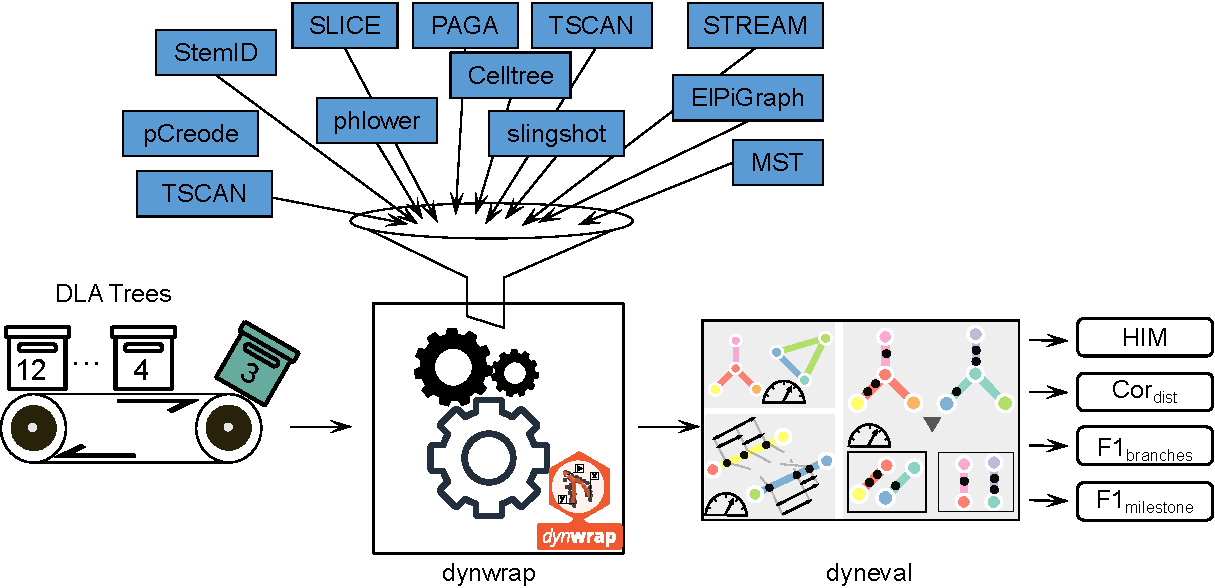
\includegraphics[width=0.95\textwidth]{evaluation_PHLOWER/fig}
	\vspace{0.1cm}
	\caption[evaluation\_PHLOWER]{
	evaluation\_PHLOWER.}
	\label{fig:evaluation_PHLOWER}
\end{figure}

\section{Technical Results}
\label{PHLOWER_bench:tech_out}
\subsection{Evaluation of Trajectory Inference Methods}

\subsubsection{Benchmarking Topology Recovery}
PHLOWER was the best-performing method in regard to tree topology recovery, followed by PAGA, RaceID/StemID and monocle~(\fref{fig:HIM}).
\begin{figure}[!h]
	\centering
	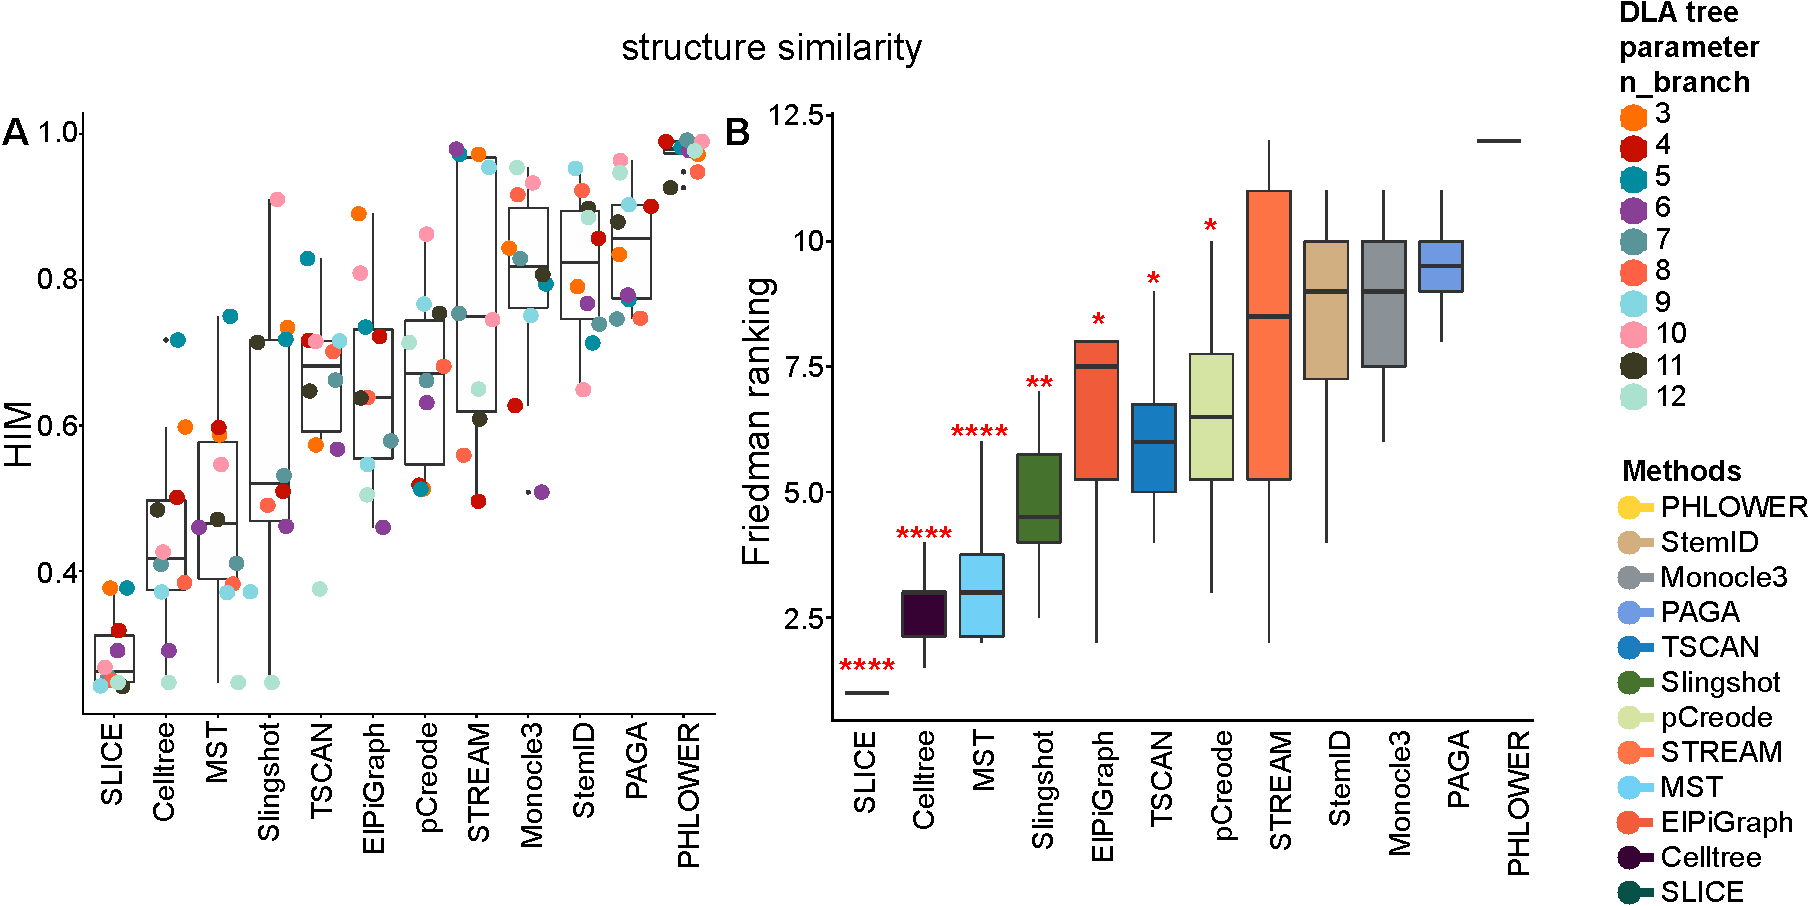
\includegraphics[width=0.95\textwidth]{HIM/fig}
	\vspace{0.1cm}
	\caption[Structure similarity benchmarking]{
	\textbf{Structure similarity benchmarking}.}
	\label{fig:HIM}
\end{figure}


\subsubsection{Benchmarking Location of cells}
In the problem of allocating cells to positions in a branch, PHLOWER was also the best performer, followed by TSCAN and RaceID/StemID~(\fref{fig:Cordist}).
\begin{figure}[!h]
	\centering
	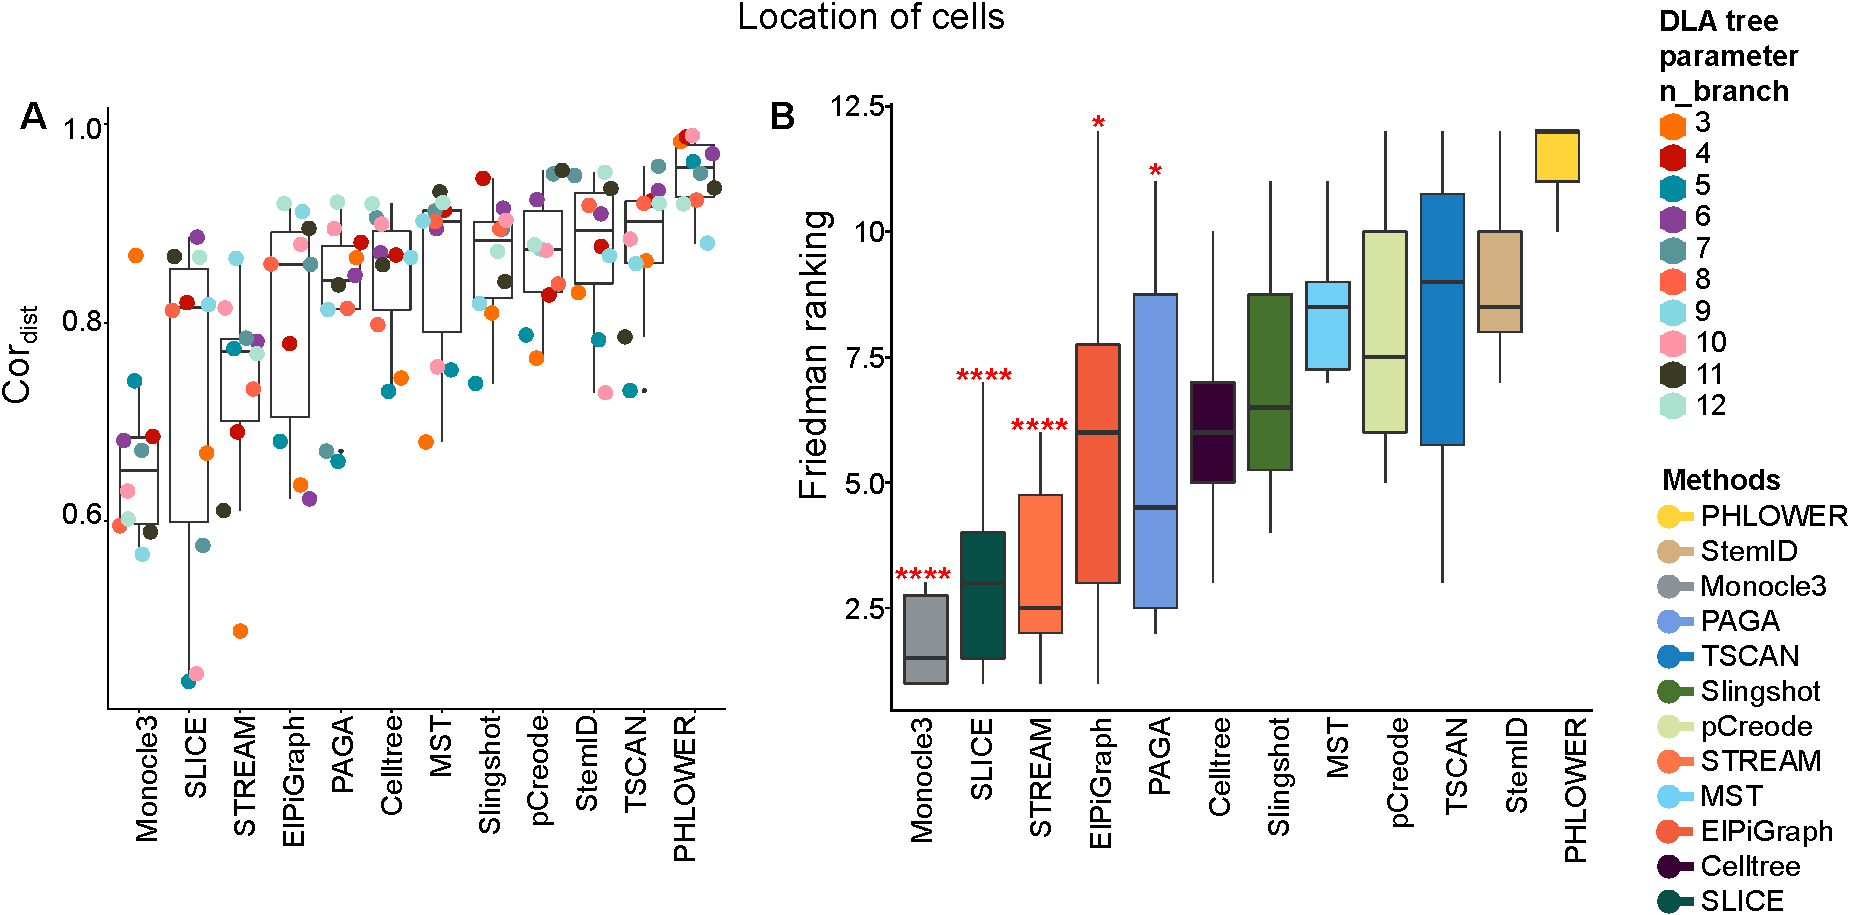
\includegraphics[width=0.95\textwidth]{Cordist/fig}
	\vspace{0.1cm}
	\caption[Location of cells]{
	\textbf{Location of cells}.}
	\label{fig:Cordist}
\end{figure}
\subsubsection{Benchmarking Branches Allocation}
In the problem of allocating cells to the correct branches, PHLOWER obtained the best performance, followed by monocle and PAGA~(\fref{fig:f1branches}).


\begin{figure}[!ht]
	\centering
	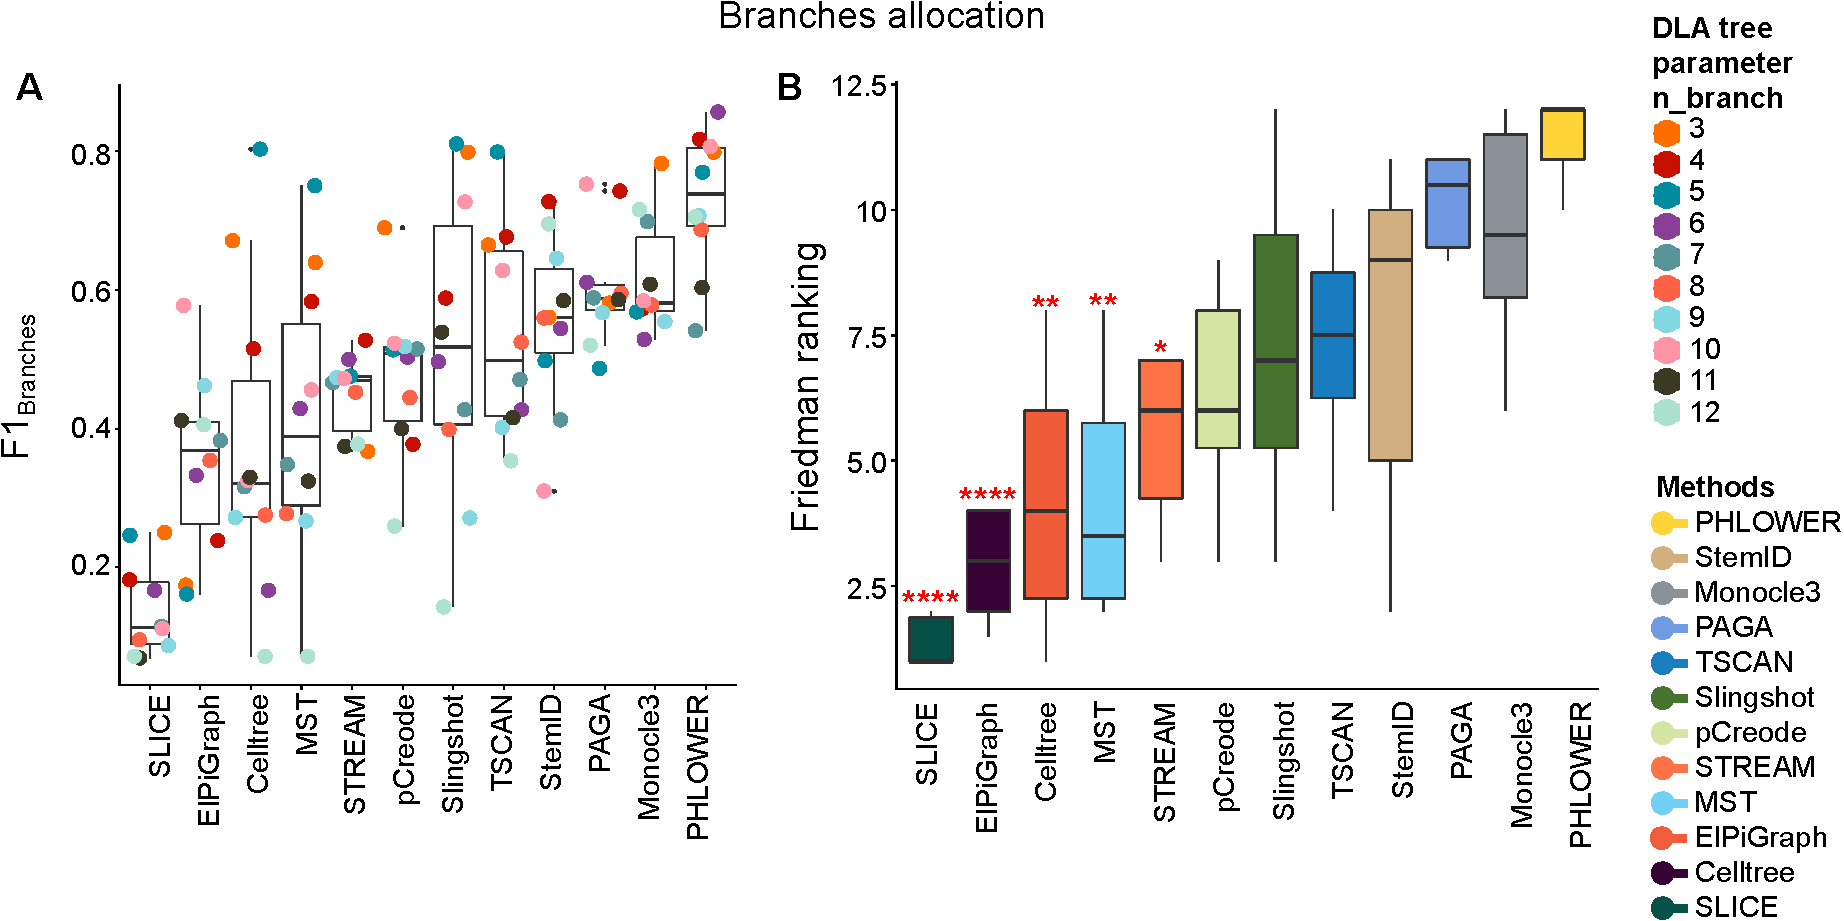
\includegraphics[width=0.95\textwidth]{F1branches/fig}
	\vspace{0.1cm}
	\caption[Branches allocation]{
	\textbf{Branches allocation}.}
	\label{fig:f1branches}
\end{figure}


\subsubsection{Benchmarking Branch points Allocation}
Finally, in the allocation of cells to branches, PHLOWER was the best performer, followed by RaceID/StemID, monocle, and PAGA~(\fref{fig:f1milestone}).
\begin{figure}[!h]
	\centering
	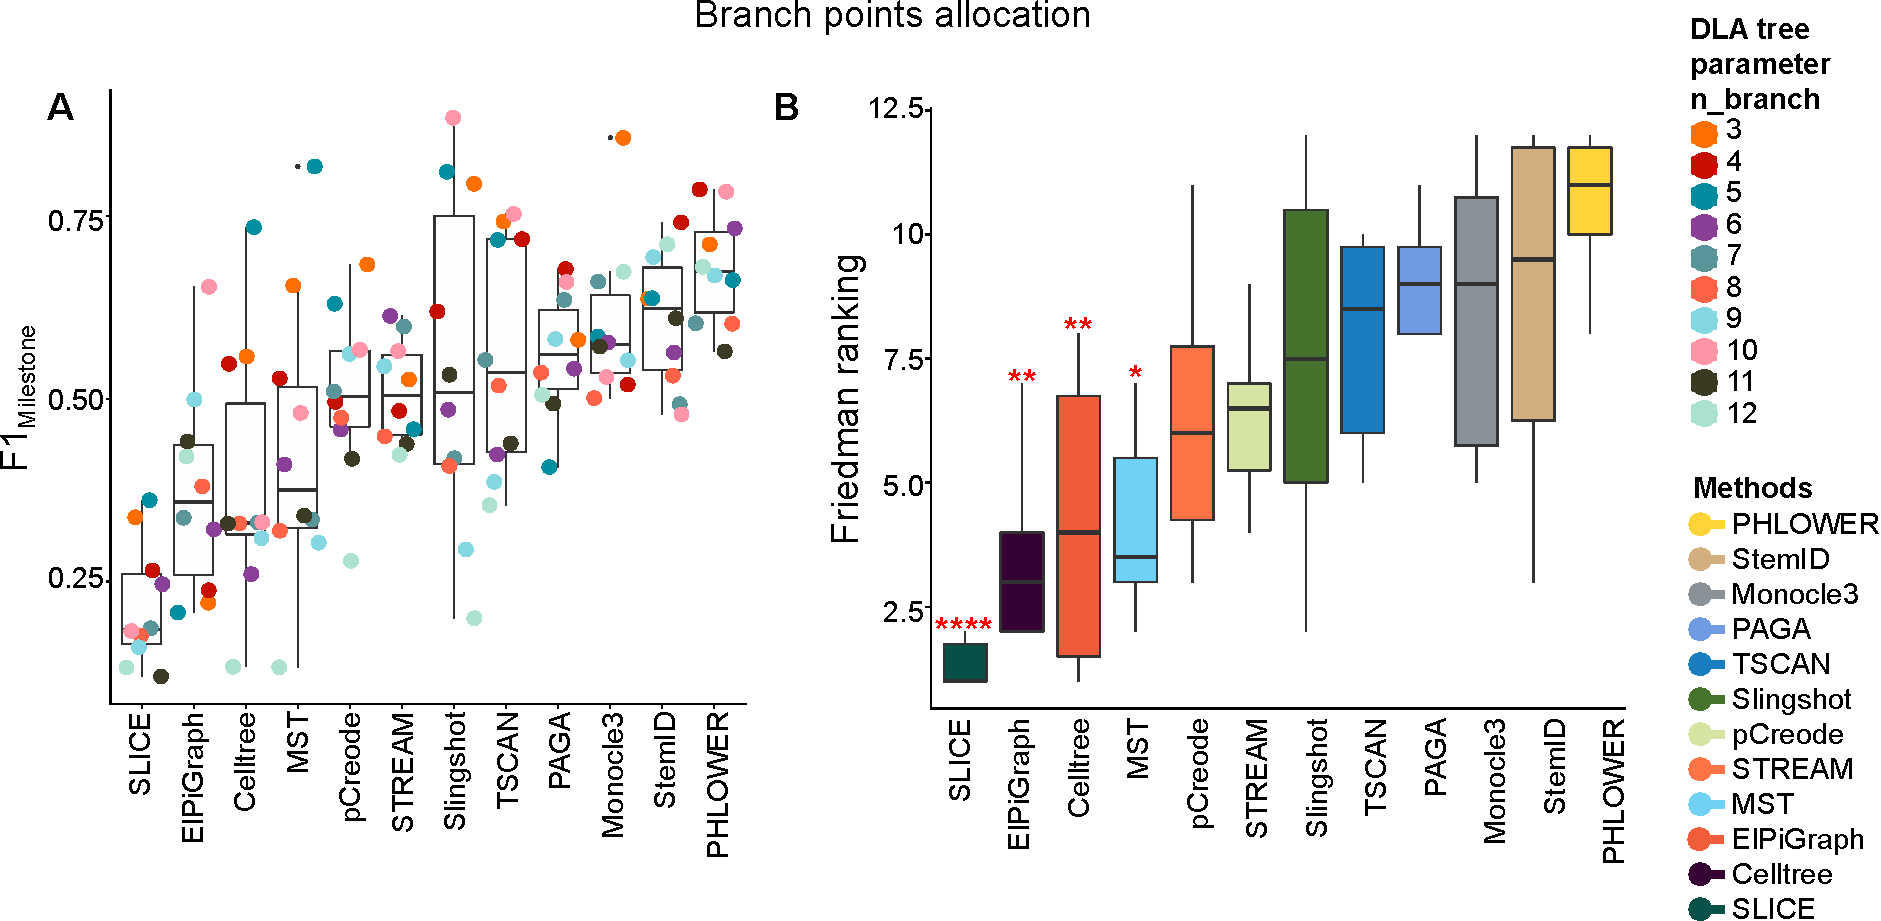
\includegraphics[width=0.95\textwidth]{F1milestone/fig}
	\vspace{0.1cm}
	\caption[Branch points allocation]{
	\textbf{Branch points allocation}.}
	\label{fig:f1milestone}
\end{figure}

\begin{figure}[!h]
	\centering
	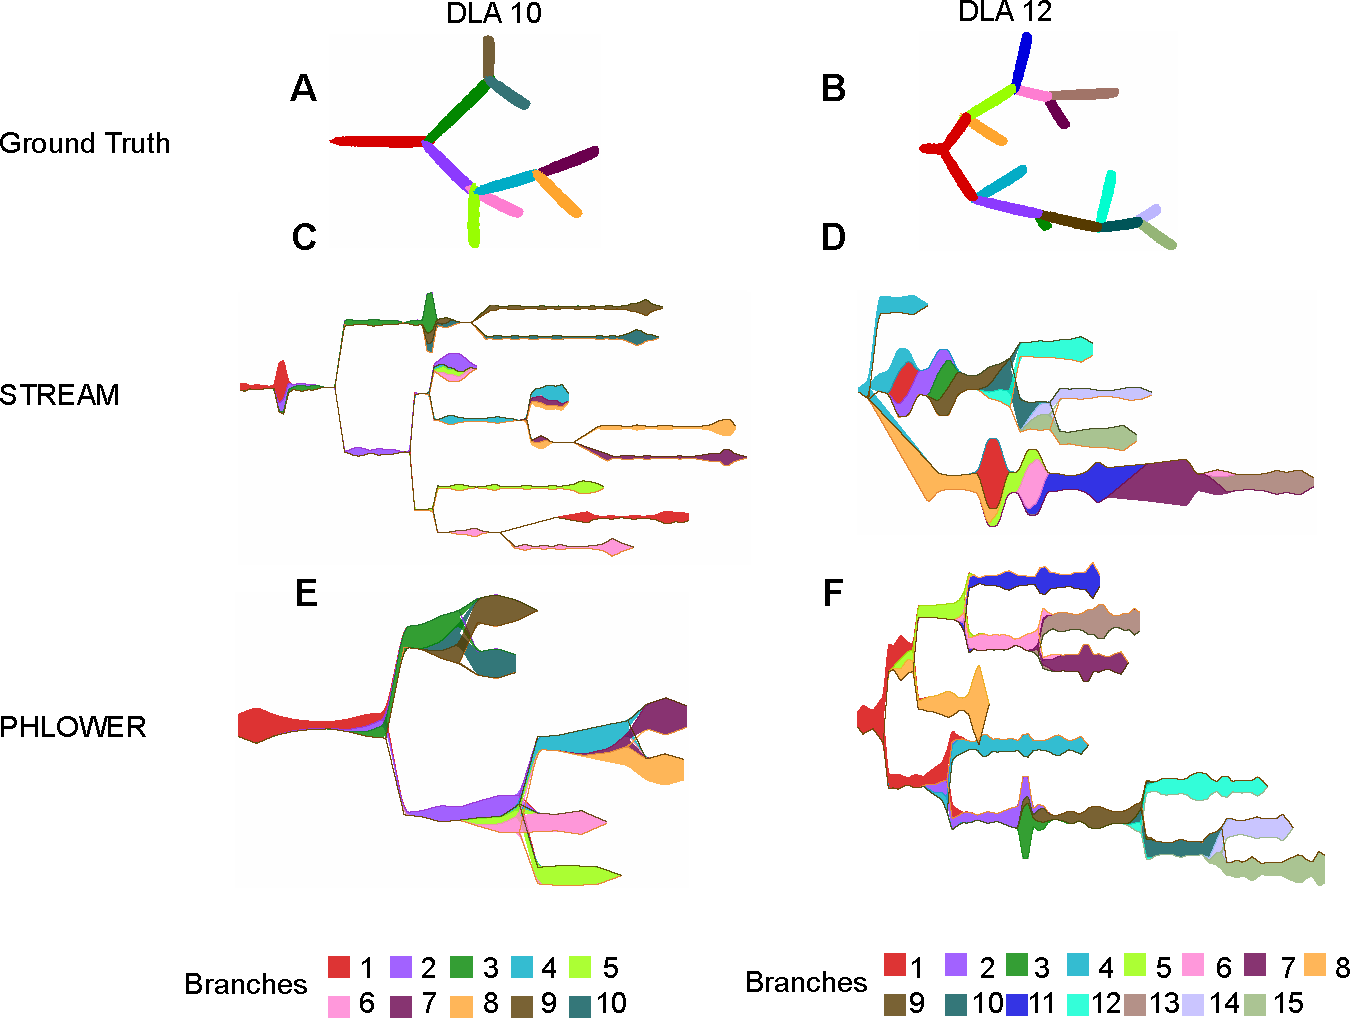
\includegraphics[width=0.95\textwidth]{PHLOWER_STREAM_layout/fig}
	\vspace{0.1cm}
	\caption[STREAM plots comparison]{
	\textbf{STREAM plots comparison}.}
	\label{fig:PHLOWER_STREAM}
\end{figure}

Altogether, PHLOWER was ranked as the top performer in all evaluated scenarios. A runner-up method was RaceID/StemID, which also ranked within the top four methods in all scenarios. The performance on PHLOWER and competing methods is illustrated by the visualisation of the tree backbones on a simulated data with six final branches as provided by dynverse~(\fref{supfig:dla10-workflow}). Moreover, graphs and embedding representations, which were produced by PHLOWER with the ten branch simulated data, represent wells PHLOWER main computational tasks


\section{Biological Experiments}
\label{PHLOWER_bench:bio_exp}
%\subsection{Experiments}
\subsection{Single Cell Kidney Organoids}

\subsubsection{Ethical statement}

Human adult skin fibroblasts derived from a healthy volunteer, after giving informed consent, were used to generate iPSCs. This study was conducted in accordance with the Helsinki Declaration as revised in 2013. Permission for the creation and use of iPSCs in this study was obtained from the local ethical commission for human-related research of the Radboud University Medical Center, Nijmegen (approval numbers: 2015-1543 and 2006-048).

\subsubsection{Cell culture}

Human adult skin fibroblasts derived from a healthy volunteer were reprogrammed into iPSCs using the Yamanaka factors~\citep{takahashi2006induction} by the Stem Cells Technology Center at Radboud University Medical Center (SCTC, Radboud UMC, Nijmegen, The Netherlands). The iPSCs used in the current study were generated from spare materials from a healthy donor, who did consent with the use of such material and did not suffer from kidney disease. The materials have been anonymized and were collected during a time in which no signed informed consent was required.

\begin{figure}[!ht]
	\centering
	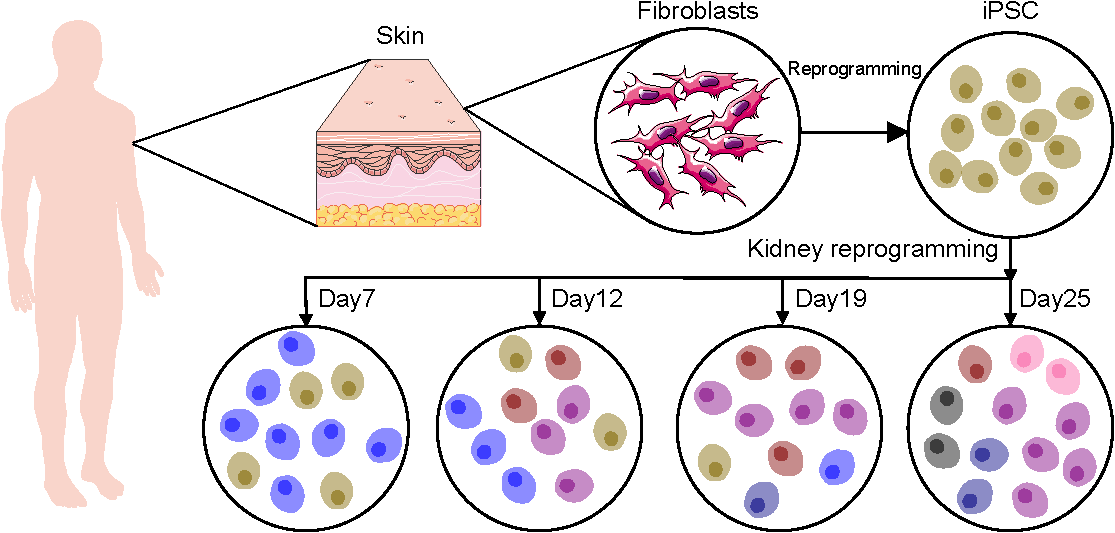
\includegraphics[width=0.75\textwidth]{Organoid_exp/fig}
	\vspace{0.1cm}
	\caption[Organoid experiment]{Organoid experiment.}
	\label{fig:organoid_exp}
\end{figure}

Generation of human induced pluripotent stem cell (iPSC) derived kidney organoids iPSC were seeded using a density of 18,000 cells/cm2 on Geltrex (Thermo Fisher, Breda, the Netherlands) coated 6-well plates (Greiner Bio-one, Alphen aan de Rijn, the Netherlands). The differentiation protocol was based on our previous work~\citep{jansen2022sars}. In brief, differentiation towards ureteric bud-like and metanephric mesenchyme lineage was initiated using CHIR-99021 (6 $\mu$M, R\&D systems, Abingdon, United Kingdom) in Essential 6 medium (Thermo Fisher, Breda, The Netherlands) for 3 and 5 days, respectively. Next, medium was  replaced sequentially for Essential 6 supplemented with fibroblast growth factor 9 (FGF9), 200 ng/ml, R\&D systems) and heparin (1 $\mu$g/ml, Sigma-Aldrich, Zwijndrecht, Netherlands) up to day 7. On day 7, differentiated cells were trypsinized and mixed in a ratio of one part 3 days CHIR-differentiated cells and two parts 5 days CHIR-differentiated cells to stimulate crosstalk between both lineages in order to boost segmented nephrogenesis. To generate cell pellets, 300,000 cells per 1.5 ml tube were aliquoted from the cell mix and centrifuged 3 times at 300 rcf for 3 min changing position by 180$^\circ$ per cycle. Cell pellets were plated on Costar Transwell filters (type 3450, Corning, Sigma-Aldrich), followed by a one-hour CHIR pulse (5 $\mu$M) in Essential 6 medium added to the basolateral compartment. Next, medium was replaced for Essential 6 medium supplemented with FGF9 and heparin for additional 5 days, and the entire 3D organoid culture was performed using the air-liquid interface. After 5 days of organoid culture, Essential 6 medium supplemented with human epidermal growth factor (hEGF, 10 ng/ml, Sigma-Aldrich), bone morphogenetic protein-7 (BMP7, 50 ng/ml, R\&D systems), stromal derived factor 1 beta (SDF1$\beta$, 10 ng/ml, R\&D systems), vasopressin (10 nM, Sigma-Aldrich), aldosterone (10 nM, Sigma-Aldrich) was used. Medium was replaced every other day for an additional 13 days.

Harvesting kidney organoids for 10x genomics NEXT GEM multiome pipeline
To dissect nephrogenic differentiation trajectories in kidney organoids using the multiome pipeline, organoids were harvested at different time points during culture. The following differentiation stages were processed:  day 7 (cells harvested from the 2D cell layer, primitive streak - intermediate mesoderm stage), organoids day 7+5, day 7+12 and day 7+18. These kidney organoid stages represent nephrogenesis ranging from intermediate mesoderm (day 7+5) towards metanephric mesenchyme and ureteric bud-like lineages (day 7+12) that result into nephron-like structures embedded by a (progenitor) stromal compartment at the end of the differentiation protocol (day 7+18). Kidney organoids were harvested on the respective dates (d7+5, d7+12, and d7+18) by cutting single organoids out of the transwell filter in a sterile flow hood using a scalpel. Organoids were washed with 5 ml PBS per filter at room temperature 3 times. Afterwards, single organoids were cut from the transwell filter with the organoids still being attached to the membrane, transferred to 1.7 ml cryovials (Greiner bio-one) and subsequently snap frozen and stored at -80$^\circ$ until nuclei isolation.

\subsubsection{Single nuclei isolation from kidney organoids}

Snap-frozen kidney organoids were thawed in PBS and crushed using a glass tube and douncer (Duran Wheaton Kimble Life Sciences, Wertheim/Main, Germany). After passing the single cell suspension through a 40 $\mu$m cell strainer (Greiner bio-one), the suspension was centrifuged at 4$^\circ C$ and 300xg for 5 min. Subsequently, the supernatant was discarded and the cell pellet was resuspended in Nuc101 cell lysis buffer (Thermo Fisher), supplemented with RNase and protease inhibitors (Recombinant RNase Inhibitor and Superase RNase Inhibitor, Thermo Fisher, and Complete Protease Inhibitor, Roche), incubated for 30 seconds and centrifuged at 4$^\circ$ and 500xg for 5 min. After discarding the supernatant, the nuclei were carefully resuspended in PBS containing 1\% (v/v) Ultra-Pure BSA (Invitrogen Ambion, Thermo Fisher) and Protector RNAse inhibitor (Sigma Aldrich). Single nuclei were counted using Trypan blue (Thermo Fisher) and prepared for 10x genomics ChromiumNextGEM Multiome pipeline v1 according to the manufacturers guidelines (~\url{https://cdn.10xgenomics.com/image/upload/v1666737555/support-documents/CG000338_ChromiumNextGEM_Multiome_ATAC_GEX_User_Guide_RevF.pdf}).


\subsubsection{Computational analysis with MOJITOO and PHLOWER}
After read mapping using the cellranger-arc tool(version 1.0.1), we filter the low-quality cells using information both from scRNA and scATAC reads. We first import scRNA to Seurat~\citep{stuart2019seurat3} to get the scRNA metrics for filtering. We next import the fragments into ArchR~\citep{granja2021archr} to get the scATAC metrics for filtering. With the information above, we retain cells with barcodes in both scRNA and scATAC count matrices. Next, we filter the cells using threshold nFeatureRNA > \num{200} \& nCountRNA <\num{400000} \&percent.mito > 5 and scATAC using thresholds in ArchR that minTSS = \num{6} \& minFrags = \num{2500} \& maxFrags = \num{1e+05}. We next perform preprocessing to scRNA using Seurat, to do this, we first normalize the scRNA data by calling NormalizeData with the default parameters, next we find top variable features with parameter selection.method='vst'. Next, we scale the data by regressing out the cell cycle and mitochondrial effect. We next run PCA with 50 PCs. To remove the batch effects, we next run harmony~\citep{korsunsky2019harmony} to integrate the four samples. For scATAC data, we use ArchR to perform the preprocessing. We first create Arrow files using the filter threshold aforementioned by calling createArrowFiles, the tile matrices are created directly from the fragment files. Next, we add doublets score by calling addDoubletScores for each sample followed by function filterDoublets to remove doublets with default parameters. Next, we run addIterativeLSI on the tile matrices to add dimensional reductions. A batch correction is also called using Harmony~\citep{korsunsky2019harmony} with function addHarmony. To obtain a uniform dimension reduction for the downstream analysis, we next run MOJITOO to integrate the scRNA and scATAC data with default parameters.

MOJITOO embedding was used as input for PHLOWER. An important parameter is the indication of the root cells. For this, we performed a clustering analysis using Seurat~\citep{stuart2019seurat3} with resolution=\num{2.5} on the MOJITOO embedding space. The root cells were defined by cluster predominantly present in day \num{7} and with the expression of mesoderm markers (TBXT, MESP1, KDR5). PHLOWER found \num{28} dimensions with zero eigenvalues and clustering analysis of the trajectory space detected 16 groups. We removed \num{4} main trajectories outliers (less than 0.5\% samples inner the cluster) and one trajectory, where cells did not further differentiated. This could be characterized by the fact that the trajectory lengths where shorter than other trajectories, i.e. trajectory length's $|skewness| > 1$.
% XXX - ok - lets talk about this to make it more clear.
Finally, some clusters had the same end time points. We therefore keep the one with the largest number of trajectories. This resulted in the \num{9} final trajectories found by PHLOWER.


\subsubsection{Regulator and Marker Selection}
We make use of the cumulative trajectory space and statistical tests to find markers and regulators associated to trajectories. Two compare two final branches, PHLOWER selects all cells associated within particular areas of the branches, i.e. highest \num{50}$\%$ of the bins. Note that every cells can be visited by several edges. To consider this important information, we multiply expression count vector of each cell by the number of visits. We then perform a statistical test (default is the $t-$test from scanpy~\citep{wolf2018scanpy}). In case we are interested in comparing sub-trees with several branches, PHLOWER first merges the sub-tree as a single branch, before the selection of the bin.

In the case of multimodal data (RNA and ATAC), PHLOWER also has a module to find regulators. First, we estimate a TF activity score per cells using chromVar~\citep{schep2017chromvar}. We then use the previously described test to find branch specific regulators. Since, TF activity cannot discern from TFs with similar motif, we only consider genes, which TF activity is similar to the expression pattern at the selected branch as in~\citep{li2023scmega}. We first get average expression/TF activity of cells of bins around the branch of interest. We next smooth the gene expression using convolution (numpy.convolve)). We then estimate the correlation between gene expression and TF activity and use this to sort branch specific regulators.

\section{Biological Results}
\label{PHLOWER_bench:bio_out}
\subsubsection{Apply Trajectory inference to kidney organoid data}

We initiated the assessment of PHLOWER's capability to infer trajectories within a single-cell multimodal dataset. To achieve this, we created a single-cell multiome kidney organoid at four distinct time points: day \num{7}, day \num{12}, day \num{19}, and day \num{25}\citep{jansen2022sars}. Following meticulous data preprocessing and quality control procedures, we successfully identified a total of \num{13751} cells, each exhibiting an average of \num{19263} fragments per cell, an average of \num{3766} detected genes, and an average of \num{10378} RNA molecules per cell~\frefp{supfig:kidney-qc}. Next, after performing dimension reduction on scRNA-seq using Seurat and scATAC-seq using ArchR, we obtained 50 PCs for scRNA and 30 iterativeLSI dimensions for scATAC-seq. Subsequently, we applied the Harmony algorithm~\citep{korsunsky2019harmony} for data correction to eliminate batch effects for both scRNA and scATAC. Following that, we employed MOJITOO to integrate the scRNA-seq and scATAC-seq data and obtained a uniform latent space with 30 dimensions. Subsequent to the integration, we conducted Louvain clustering with resolution=2.5 in the MOJITOO space, resulting in a total of \num{31} clusters.

\begin{figure}[!h]
	\centering
	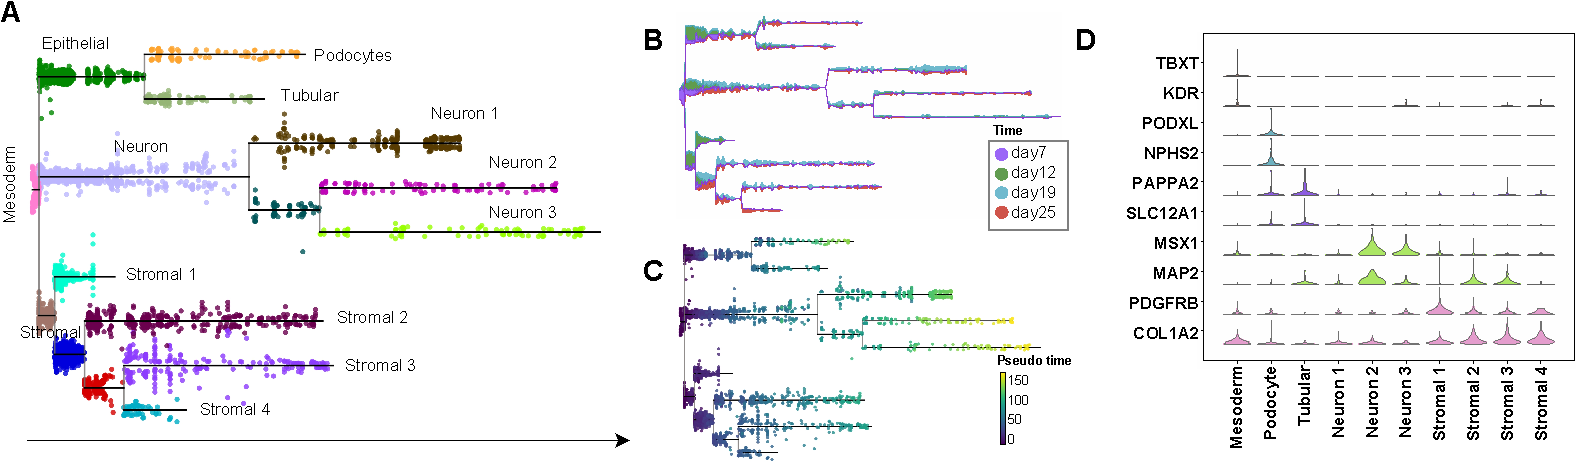
\includegraphics[width=0.95\textwidth]{kidney_main/fig}
	\vspace{0.1cm}
	\caption[Annotation of Kidney Orgnoid Data]{\textbf{Annotation of Kidney Orgnoid Data}. \textbf{A)} Differentiation tree on the kidney organoid data as estimated by PHLOWER. \textbf{B-C)} Day of experiments and pseudo-time estimates of cells in the differentiation trees. \textbf{D)} Violin plot with marker of end branches}
	\label{fig:kidney_organoid}
\end{figure}

Next, We provided the data as input for PHLOWER, which recovered a trajectory with nine branches~(\fref{fig:kidney_organoid}A,~\afref{supfig:kidney-workflow}). We observe that the tree successfully sorts cells regarding the organoids age~(\fref{fig:kidney_organoid}B) and this matches well with the pseudo-time estimates~(\fref{fig:kidney_organoid}C). The nine branches were associated with three major branches associated with epithelial cells (two branches associated with podocytes and tubular cells); stromal cells (four branches) and a major branch associated with muscle and neuronal cells (3 branches). The identity of these cells is revealed by the expression of markers as TBXT~\citep{schmidt2016grow} and KDR~\citep{evseenko2010mapping} for mesoderm cells;  PODXL~\citep{Menon2018} and NPHS2~\citep{Menon2018} for podocytes, SLC12A1~\citep{Hochane2019} and PAPPA2~\citep{Hochane2019} for kidney tubular cells;  COL1A2~\citep{Menon2018} and PDGFRA~\citep{Combes2019} for stromal cells; and neuronal and muscle markers RFX4~\citep{jansen2022sars} and MSX1~\citep{Combes2019,Hochane2019,Menon2018,schmidt2016grow}. The latter branch are considered off target cells and potentially represents non-fully differentiated cells, which should be present in kidney organoids.


\begin{figure}[!h]
	\centering
	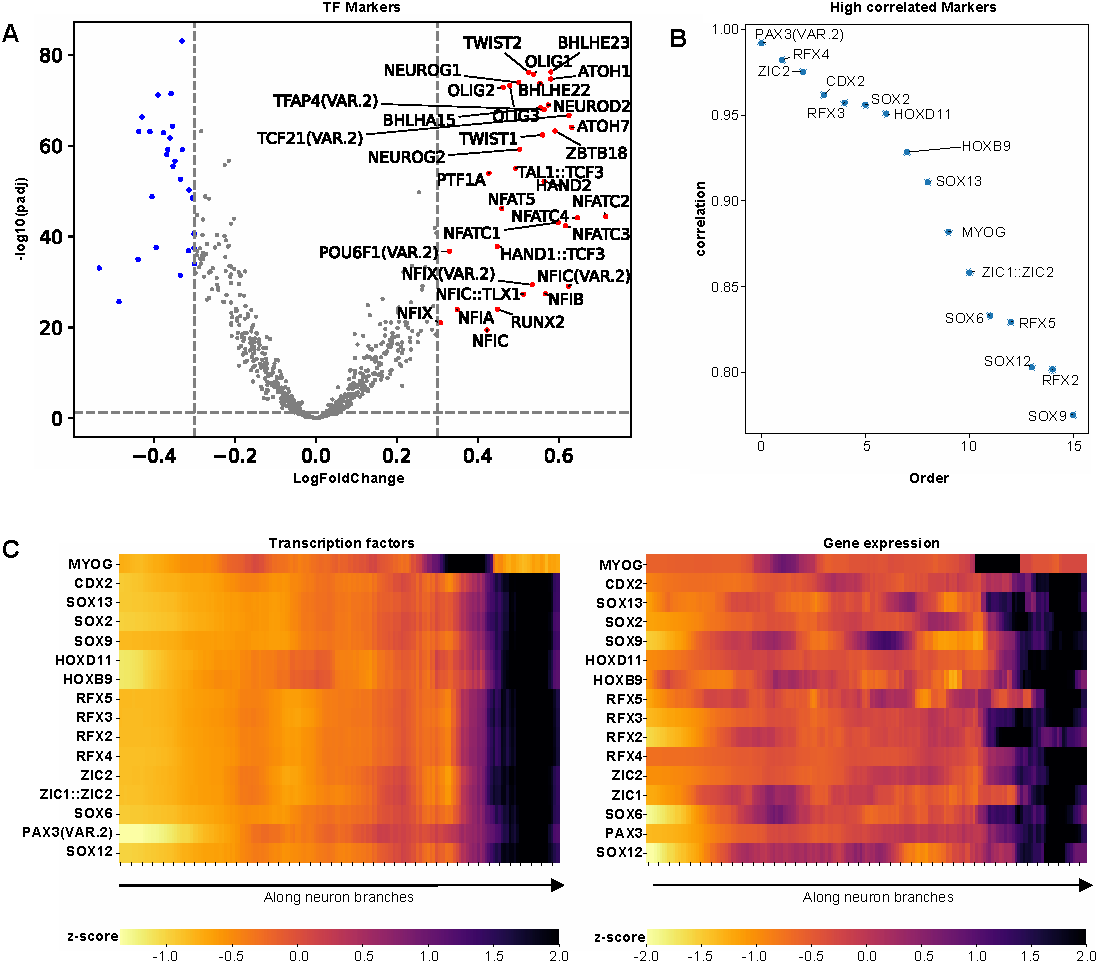
\includegraphics[width=0.95\textwidth]{Neuron_TF_diff/fig}
	\vspace{0.1cm}
	\caption[Neuron branches TF differentiation]{\textbf{Neuron branches TF differentiation}. \textbf{A)} vocano. \textbf{B)}rank. \textbf{C)} correlated heatmap}
	\label{fig:Neuron_TF_diff}
\end{figure}


A key question to be addressed by PHLOWER is regulators (transcription factors; TF) driving the differentiation of organoids. We leverage here both the trees inferred by PHLOWER to find TFs related to branch differentiation using a procedure similar to scMega~\citep{li2023scmega}. In short, we estimated TF activity scores with ChromVAR~\citep{schep2017chromvar} and selected TFs, which expression are concordant with the TF activity and are differential expressed between compared branches~(\fref{supfig:TF-diff}). When comparing cells in the end of tubular and podocyte trajectories, this recover bonafide regulators of these cells such as WT1~\citep{kann2015genome} and MAFB~\citep{schreibing2022mapping} for podocytes and HNF1B~\citep{kompatscher2017loss} and GRHL2~\cite{aue2015grainyhead} for tubular cells~\frefp{supfig:kidney-markers}. Next, we compared major branches: stromal cells vs. others and neuronal/muscle cells vs. others. We detected TWIST1 and RUNX2 are regulators of stromal cells and PAX3, RFX4 and ZIC2 as regulators of neuronal/muscle cells~\frefp{fig:Neuron_TF_diff}.


\subsubsection{Characterize the cell fate xxxx}

\section{statistical}
\label{PHLOWER_bench:statistical}

For comparisons involving multiple methods and datasets, we employed the non-parametric Friedman test with the Nemenyi post-hoc test (Demšar, 2006). The Friedman test(Friedman, 1937, 1940) was utilized to compare the average ranks of the methods across all datasets. The null hypothesis assumes that all the methods are equivalent, and their ranks are equal. We utilized the friedmanTest function from the R package PMCMRplus to conduct the Friedman rank sum test. If the null hypothesis was rejected, indicating that at least one method is significantly different from the others, we proceeded with the Nemenyi post-hoc test (Nemenyi, 1963) to compare all pairs. Therefore, to compare k methods, a total of $k(k-1)/2$ hypotheses were tested, and this was accomplished using the frdAllPairsNemenyiTest function from the R package PMCMRplus.



\section{Discussion}
\label{PHLOWER_bench:discussion}

In this chapter, we first described the experimental framework and to evaluate our computational trajectory inference method from technical points of view~\srefp{PHLOWER_bench:tech_exp}. We introduced a simulation algorithm to generate tree structure datasets with different numbers of branches. Next, we provided the full details of the execution and parameterization of the competing methods. We also introduced different metrics from the dynverse trajectory inference evaluation system. Next, we presented the result of the technical validation\srefp{PHLOWER_bench:tech_out}. The benchmarking shows that PHLOWER outperforms in four metrics: topology recovery, location of cells, branch allocation, and branch points allocation.

To validate the biological performance of PHLOWER, we then described the biological experiment design and validation results. We generated novel single-cell multimodal data from human organoids to derive kidney lineage with four time points: day 7, day 12, day 19, and day 25. Next, we applied MOJITOO to perform integration and PHLOWER to produce a 9-end-branches differentiation tree. With PHLOWER, we were able to identify the transcription factors that regulated off-target cells. xxxx


